\documentclass{bioinfo}
\copyrightyear{2016} \pubyear{2016}

\usepackage{graphicx}
\usepackage{caption}
\usepackage{subfigure}


\access{Advance Access Publication Date: Day Month Year}
\appnotes{Databases and ontologies}

\begin{document}
\firstpage{1}

\subtitle{Databases and ontologies}

\title[RTCGA Family of R packages]{RTCGA - The Family of R Packages Integrating Data from The Cancer Genome Atlas Study}
\author[Marcin Kosi\'nski \textit{et~al}.]{Marcin Kosi\'nski\,$^{\text{\sfb 1,2,}*}$, Witold Chodor\,$^{\text{\sfb 2}}$ and Przemys\l{}aw Biecek\,$^{\text{\sfb1,2}}$}
\address{$^{\text{\sf 1}}$Faculty of Mathematics and Information Science, Warsaw University of Technology, 00-662 Warsaw, Poland and \\
$^{\text{\sf 2}}$Faculty of Mathematics, Informatics, and Mechanics, University of Warsaw, City, 02-097 Warsaw, Poland.}

\corresp{$^\ast$To whom correspondence should be addressed.}

\history{Received on XXXXX; revised on XXXXX; accepted on XXXXX}

\editor{Associate Editor: XXXXXXX}

\abstract{\textbf{Summary:} 
We present a family of \textbf{R} packages called \textbf{RTCGA} that simplify access to data from the TCGA project.
The Cancer Genome Atlas Project (TCGA) is a coordinated effort to accelerate the understanding of the molecular basis of cancer. It is a source of curated multi-platform data, including RNA-seq, DNA-seq, DNA Methylation, together with clinical data for over 11 thousand patients and 33 cancer types. This rich source of data is accessible in raw format from TCGA Data Portal. \textbf{RTCGA} packages facilitate access to these datasets, streamline merging characteristics from different platforms and support exploratory statistical analyses and visualizations. \\
\textbf{Availability:} \textbf{RTCGA} family of \textbf{R} packages is freely available at GitHub http://rtcga.github.io/RTCGA/ and from
the  Bioconductor  project  at  http://bioconductor.org/packages/RTCGA/ .\\
\textbf{Contact:} \href{m.p.kosinski@gmail.com}{m.p.kosinski@gmail.com}}


\maketitle

\begin{figure*}
\center
	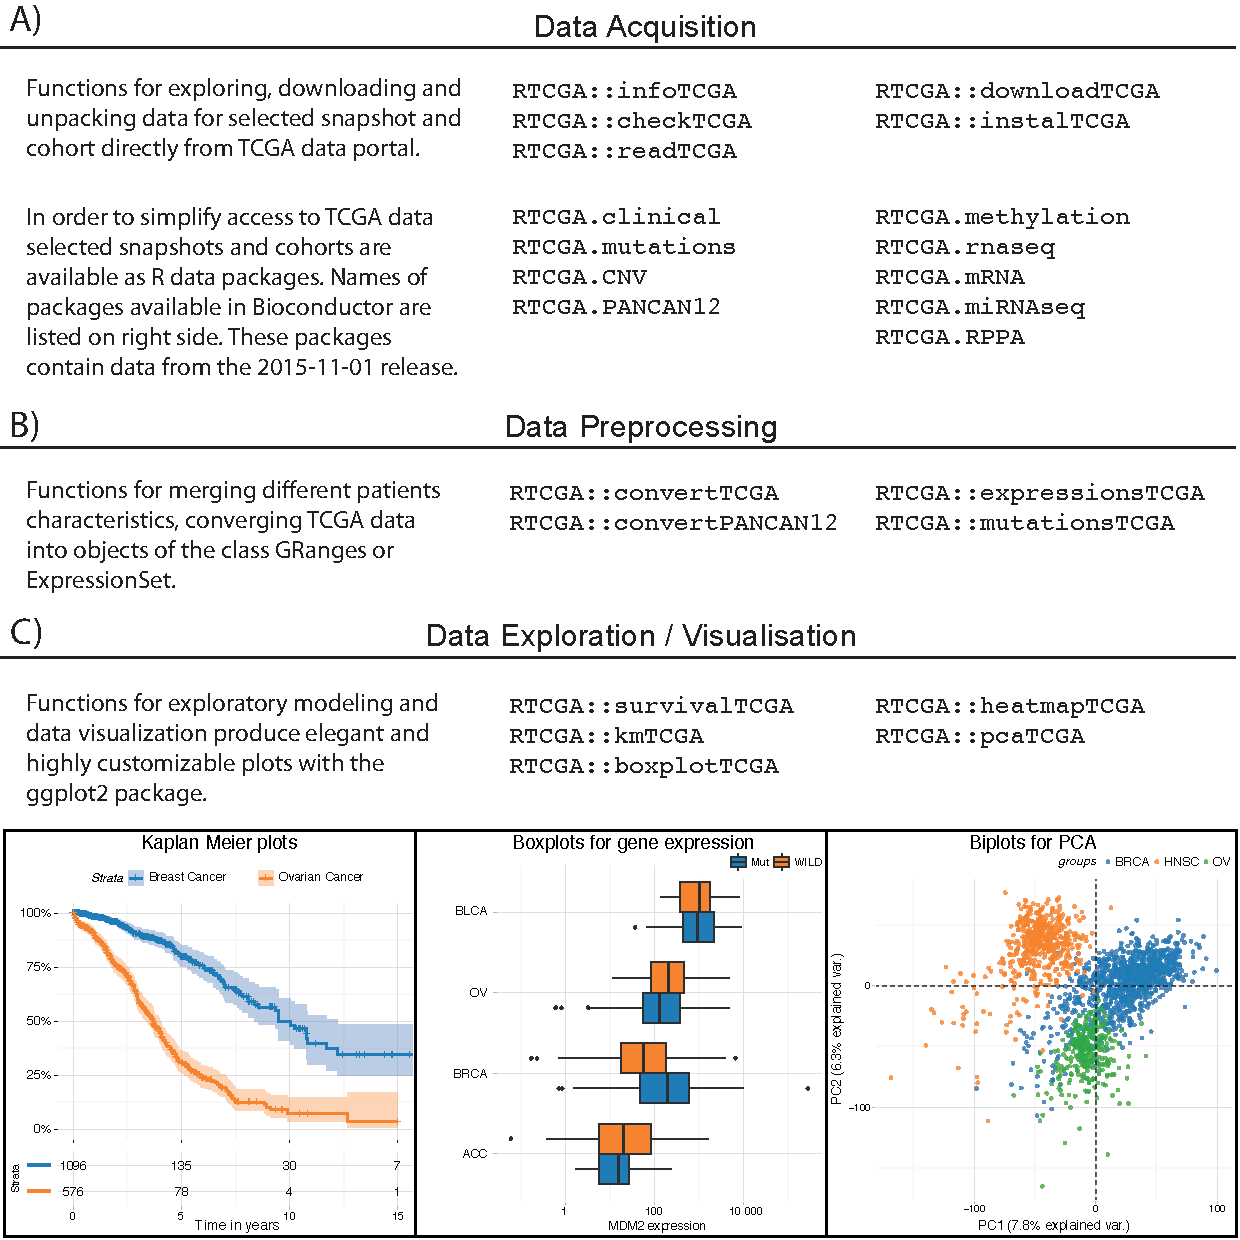
\includegraphics[width=0.9\linewidth]{figures/RTCGA.pdf}
	\caption{The architecture of \textbf{RTCGA} family of R packages. (A) The \textbf{RTCGA} package contains functions for exploration of TCGA metadata for all available releases; function that allows to download every dataset from TCGA study and functions that enables to read data into the tidy format. In addition to this package a set of data packages are available in Bioconductor. (B) Data.frames with data from specific platform can be converted to Bioconductor format (\texttt{ExpressionSet, GRanges}) or merged with data from different platforms. (C) 
The \textbf{RTCGA} package also contains functions for exploratory analyses of TCGA data along with some popular visualisations. In this example following statistics are presented: Kaplan-Meier estimates of survival curves and risk set table for \textbf{Breast invasive carcinoma (BRCA)} and \textbf{Ovarian serous cystadenocarcinoma (OV)} cohorts; Boxplot for samples with mutated of wild-type versions of MDM2 gene; Principal Component Analysis performed for genes expressions (RNASeq) for \textbf{Breast invasive carcinoma (BRCA)}, \textbf{Head and Neck squamous cell carcinoma (HNSC)} and \textbf{Ovarian serous cystadenocarcinoma (OV)} cohorts}.}
\label{fig:RTCGA_workflow_ver3}
\end{figure*}


\subsubsection*{Introduction}
\cite{TCGAP} provides a platform for researchers to search, download, and analyze data sets generated by TCGA Project. It contains clinical information, genomic characterization data, and high level sequence analysis of the tumor genomes for 11 thousands patients, over 2.5 PT of data. Compressed \textit{tar.gz} files are available through \cite{BroadGDAC} and recently through \cite{GDC}. One can select a release (monthly snapshots), cancer type (cohort) and data type (e.g. clinical, RNA expression, methylation) and download a text file with raw data. 

While working with many cohorts and cancer types we found this approach burdensome. Without easy-to-use API it is harder to reproduce results obtained in past.
\begin{itemize}
\item If one requires to download datasets containing e.g. information about genes' expressions for all available cohorts types, then one would have to go through the click-to-download process separately for each cohort. This is inconvenient and time-consuming.
\item Some datasets (e.g. clinical) are not in a standard tidy data format, which is: one row for one observation and one column for one variable. Data for some platforms data is transposed (e.g. for expression columns stands for patients) for others data is unstructured (e.g. mutations). That becomes more onerous when investigating many clinical datasets at once.
\item Data governance for many datasets for various cohorts saved in different folders with very long names may be exhausting and uncomfortable for researchers that are not very skilled in data management or data processing.
\end{itemize}
For reasons listed above we prepared an uniform API to download and pre-process selected datasets along with set of R data packages with pre-processed data. 
The prepared packages are useful for biostatisticians that work with cancer data along with researchers that work on scalable big data algorithms or lecturers that are are using real world case studies.

\subsubsection*{Using RTCGA packages}
The general architecture of all packages in the \textbf{RTCGA} family is presented in the Figure 1a. All packages listed in this figure are available at Bioconductor.
The software package \textbf{RTCGA} contains functions that facilitate download of data from particular date, cohort and platform. Other functions benefits data processing, analysis and visualizations. In figures 1b-1c we present example analyses and plots that cover Kaplan-Meier estimates of survival curves and Principal Component Analysis. Detailed instructions on how to apply these and other analyses, and on how to download the selected data are presented at the project's website. Different versions of data packages refer to particular snapshots of the data. 


\subsubsection*{Acknowledgements}
This work was supported by NCN Grant 2016/21/B/ST6/02176.

\bibliographystyle{natbib}
%\bibliographystyle{achemnat}
%\bibliographystyle{plainnat}
%\bibliographystyle{abbrv}
%\bibliographystyle{bioinformatics}
%
%\bibliographystyle{plain}
%
\bibliography{main}


\end{document}
